\documentclass[a4paper]{article}
\usepackage{fullpage}
\usepackage{mathptmx}
\newcommand{\mse}[0]{\texttt{monitored-session-erlang}}
\usepackage{url}
\usepackage{parskip}
\usepackage[scaled=0.7]{beramono}
\usepackage[numbers]{natbib}
\usepackage{graphicx}
\usepackage{listings}
\usepackage{float}
\newcommand{\msechat}[0]{\texttt{mse-chat}}
\usepackage{listings}
\usepackage{upquote}
\usepackage{color}

\definecolor{bluekeywords}{rgb}{0.13,0.13,1}
\definecolor{greencomments}{rgb}{0,0.5,0}
\definecolor{turqusnumbers}{rgb}{0.17,0.57,0.69}
\definecolor{redstrings}{rgb}{0.5,0,0}

\lstdefinelanguage{Scribble}{
  morekeywords={
  	global, protocol, role, from, to, interruptible, with, do, instantiates, par, and, rec, continue, choice, at, initiates, handle, returning, call, local, or
  },
  otherkeywords={ },
  keywordstyle=\color{bluekeywords},
  sensitive=true,
  %basicstyle=\scriptsize\ttfamily,
  basicstyle=\linespread{0.9}\ttfamily,
	breaklines=true,
  xleftmargin=\parindent,
  belowskip=\bigskipamount,
  aboveskip=\bigskipamount,
  tabsize=4,
  morecomment=[l][\color{greencomments}]{///},
  morecomment=[l][\color{greencomments}]{//},
  morecomment=[s][\color{greencomments}]{{(*}{*)}},
  morestring=[b]",
  showstringspaces=false,
  literate={`}{\`}1,
  frame=none,
  showlines=false,
  frame=single,
  stringstyle=\color{redstrings},
}

\lstset{
  language=Scribble,
  showstringspaces=false,
  formfeed=\newpage,
  tabsize=2,
  commentstyle=\itshape,
  basicstyle=\linespread{0.9}\ttfamily,
  %captionpos=b,
  %belowcaptionskip=4pt,
}
% \renewcommand*\familydefault{\ttdefault} %% Only if the base font of the document is to be typewriter style
\usepackage[T1]{fontenc}

\title{Erlang Chat Server}
\author{Simon Fowler}
\begin{document}
\maketitle

\section{Introduction}
In this report, we describe the design and implementation of a session-typed chat server, \msechat{}, using the \mse{}~\cite{fowler:msc} session types framework for the Erlang programming language.

More of an introduction to the \mse{} framework is contained within the DNS Server case study.

\section{Description}
\msechat{} is a chat server built on the \mse{} framework. The structure of the application follows standard Erlang/OTP practices, and is arranged in a supervision tree. The supervision tree is shown in Figure~\ref{edns-supervision-tree}.

\begin{figure}[htpb]
\centering
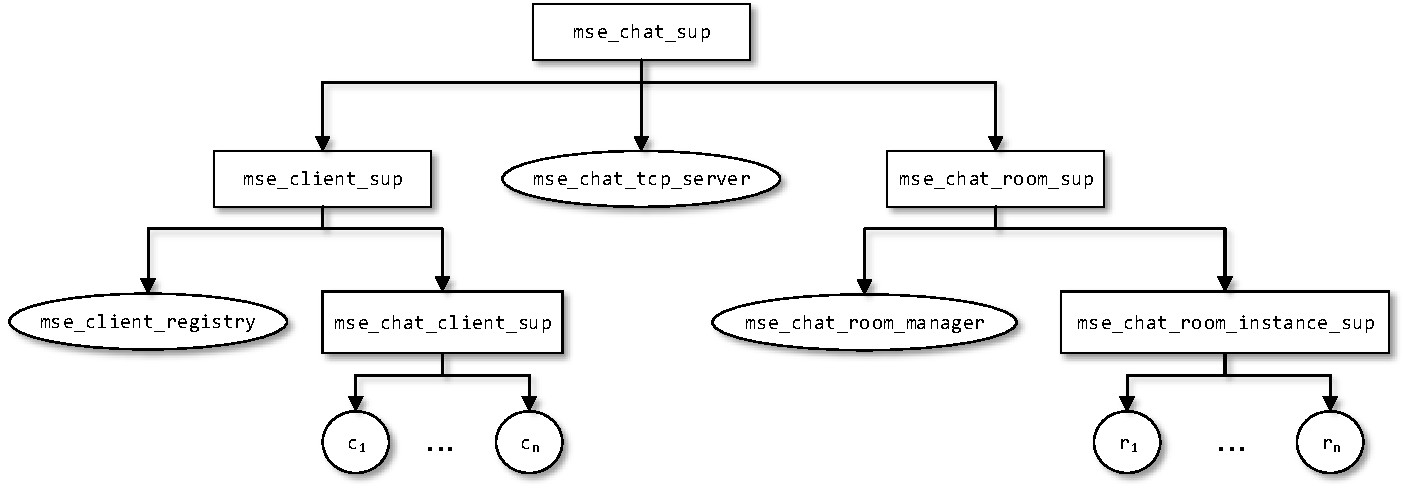
\includegraphics[width=0.8\textwidth]{MSE-Chat-Tree.pdf}
\label{edns-supervision-tree}
\caption{Supervision Tree for \texttt{mse-chat}}
\end{figure}

As is typical, we have a root supervisor, \texttt{mse-chat-sup}. We have two subsystems: a client subsystem, consisting of a client registry and a client supervisor: the client supervisor spawns child processes to handle communication with the user, but does not restart them should they fail. The \texttt{mse\_chat\_tcp\_server} listens on a socket and accepts new clients, spawning a new \texttt{mse\_chat\_client} when a client connects.

Clients can create and join chat rooms. Chat rooms are represented by \texttt{mse\_chat\_room\_instance} actors and recorded by the \texttt{mse\_chat\_room\_manager} actor. 

Excluding supervisors, the different types of actors are as follows:

\begin{description}
\item[\texttt{mse\_chat\_client} (written as $c_1$ \ldots $c_n$)] \hfill \\
An actor spawned for each chat client. Contains the socket used to communicate with the client.
\item[\texttt{mse\_chat\_tcp\_server}] \hfill \\
Listens on a socket, and spawns a new \texttt{mse\_chat\_client} actor when a new connection is made.
\item[\texttt{mse\_chat\_room\_instance} (written as $r_1$ \ldots $r_n$)] \hfill \\
Represents a chat room. Contains details about the current clients joined to the chat room, and can register / deregister clients, and broadcast chat messages.
\item[\texttt{mse\_chat\_room\_manager}] \hfill \\
A registry for chat rooms. Stores a mapping from chat room name to process ID. Can create, lookup, and list chat rooms.
\end{description}

The protocol proceeds as follows:

\begin{itemize}
\item A client connects to the server.
\item An \texttt{mse\_chat\_client} actor is spawned to handle incoming requests from the new client.
\item A client can either create or join a room. 
\begin{itemize}
\item If a client chooses to create a room, it sends a request to \texttt{mse\_chat\_room\_manager}, which responds by either notifying the client that the room has been created successfully, or that the room already exists.
\item If a client chooses to join a room, it sends a request to \texttt{mse\_chat\_room\_manager} to ascertain whether the room exists. If so, then the client is registered with the room. Once registered with the room, any chat messages sent should be delivered to all other clients registered with the room.
\end{itemize}
\item The client can leave the session at any time. When it leaves, it should be deregistered from any rooms to which it is registered.
\end{itemize}

The chat server example differs from the DNS server as sessions are longer: whereas a DNS handling session existed only while the request was being fulfilled, a chat server persists for as long as the client remains connected to the server. Similarly to the DNS server example, not all roles are inhabited at the start of the protocol, as a client joins the chat room only after specifying the room name.

Upon receiving the room PID, the client creates a new subsession for interactions within the chat room. In this session, it is important to note that communication is \emph{bidirectional}: the client can send chat messages to the chat room, and can also receive messages from the chat room. When a user sends a chat message to the room, it should be broadcast to all participants of the room. This is encoded using the \texttt{par} block, where each scope contains actions that can be performed in an interleaved fashion. 

The subsession initiation is implemented using the custom \texttt{initiates} construct: 

\begin{lstlisting}[language=scribble]
Role initiates ProtocolName(Roles) { SuccessBlock } handle(FailureName) { FailureBlock } 
\end{lstlisting}

The \texttt{initiates} construct initiates a subsession for the protocol \texttt{ProtocolName} with the given roles (in this case, \texttt{ClientThread} is an internal invitation, inviting the actor playing the \texttt{ClientThread} role in \texttt{ChatServer} to play the \texttt{ClientThread} role in \texttt{ChatSession}, and an external invitation for another actor to play the \texttt{ChatRoom}).

The \texttt{SuccessBlock} block describes the interactions to occur should the subsession complete successfully, whereas the \texttt{handle} constructs allow different interactions to take place should the subsession terminate abnormally. In this case, we allow a client to join a different room should the chat room go offline (note that \texttt{ParticipantOffline} is the error raised when an actor in a subsession is terminated while it is still needed in the subsession).

A participant may disconnect at any time. If this is the case, then they should be deregistered from any chat rooms to which they belong.

\section{Scribble Protocol}

We specify the communication within the system using two protocols: \texttt{ChatServer}, which describes the interactions prior to joining a chat room, and \texttt{ChatSession}, which describes the interactions within the chat session. The session types are written in the Scribble protocol description language~\cite{honda:scribble,scribblespec}.

\begin{minipage}{\linewidth}
\begin{lstlisting}[language=scribble]
module src.com.simonjf.ScribbleExamples.ChatServer.ChatServer;

type <erlang> "string" from "" as Username;
type <erlang> "string" from "" as Password;
type <erlang> "tuple" from "" as ClientData;
type <erlang> "string" from "" as String;
type <erlang> "string" from "" as RoomName;
type <erlang> "list" from "" as StringList;
type <erlang> "string" from "" as PID;


global protocol ChatServer(role ClientThread, role RoomRegistry) {
    rec ClientChoiceLoop {
        // When not in a room, a user can either join, create, or list the rooms.
        choice at ClientThread {
            lookupRoom(RoomName) from ClientThread to RoomRegistry;
            choice at RoomRegistry {
                roomPID(RoomName, PID) from RoomRegistry to ClientThread;
                ClientThread initiates ChatSession(ClientThread, new ChatRoom) {
                    continue ClientChoiceLoop;
                } handle (ParticipantOffline) {
                      continue ClientChoiceLoop;
                }
            } or {
                roomNotFound(RoomName) from RoomRegistry to ClientThread;
            }
        } or {
            createRoom(RoomName) from ClientThread to RoomRegistry;
            choice at RoomRegistry {
                createRoomSuccess(RoomName) from RoomRegistry to ClientThread;
            } or {
                roomExists(RoomName) from RoomRegistry to ClientThread;
            }
        } or {
            listRooms() from ClientThread to RoomRegistry;
            roomList(StringList) from RoomRegistry to ClientThread;
        }
        continue ClientChoiceLoop;
    }
}

global protocol ChatSession(role ClientThread, role ChatRoom) {
    // Communication is bidirectional: a client can send messages to the
    // server (either chat messages or control messages), and the server
    // can send messages to the client (incoming chat messages)
    par {
        rec ClientLoop {
            choice at ClientThread {
                outgoingChatMessage(String) from ClientThread to ChatRoom;
                continue ClientLoop;
            } or {
                leaveRoom() from ClientThread to ChatRoom;
            }
        }
    } and {
        rec ServerLoop {
            incomingChatMessage(String) from ChatRoom to ClientThread;
            continue ServerLoop;
        }
    }
}
\end{lstlisting}
\end{minipage}

\subsection{Local Projections}
\subsubsection{ClientThread}
\begin{lstlisting}[language=scribble]
module src.com.simonjf.ScribbleExamples.ChatServer.ChatServer_ClientThread;

type <erlang> "string" from "" as Username;
type <erlang> "string" from "" as Password;
type <erlang> "tuple" from "" as ClientData;
type <erlang> "string" from "" as String;
type <erlang> "string" from "" as RoomName;
type <erlang> "list" from "" as StringList;
type <erlang> "string" from "" as PID;

local protocol ChatServer at ClientThread(role ClientThread,role RoomRegistry) {
    rec ClientChoiceLoop {
        choice at ClientThread {
            lookupRoom(RoomName) to RoomRegistry;
            choice at RoomRegistry {
                roomPID(RoomName,PID) from RoomRegistry;
                ClientThread initiates ChatSession( ClientThread , new ChatRoom ) {
                    continue ClientChoiceLoop;
                } handle (ParticipantOffline) {
                    continue ClientChoiceLoop;
                }
            } or {
                roomNotFound(RoomName) from RoomRegistry;
            }
        } or {
            createRoom(RoomName) to RoomRegistry;
            choice at RoomRegistry {
                createRoomSuccess(RoomName) from RoomRegistry;
            } or {
                roomExists(RoomName) from RoomRegistry;
            }
        } or {
            listRooms() to RoomRegistry;
            roomList(StringList) from RoomRegistry;
        }
        continue ClientChoiceLoop;
    }
}

local protocol ChatSession at ClientThread(role ClientThread,role ChatRoom) {
    par {
        rec ClientLoop {
            choice at ClientThread {
                outgoingChatMessage(String) to ChatRoom;
                continue ClientLoop;
            } or {
                leaveRoom() to ChatRoom;
            }
        }
    } and {
        rec ServerLoop {
            incomingChatMessage(String) from ChatRoom;
            continue ServerLoop;
        }
    }
}
\end{lstlisting}
\subsubsection{RoomRegistry}
\begin{lstlisting}[language=scribble]
module src.com.simonjf.ScribbleExamples.ChatServer.ChatServer_RoomRegistry;

type <erlang> "string" from "" as Username;
type <erlang> "string" from "" as Password;
type <erlang> "tuple" from "" as ClientData;
type <erlang> "string" from "" as String;
type <erlang> "string" from "" as RoomName;
type <erlang> "list" from "" as StringList;
type <erlang> "string" from "" as PID;

local protocol ChatServer at RoomRegistry(role ClientThread,role RoomRegistry) {
    rec ClientChoiceLoop {
        choice at ClientThread {
            lookupRoom(RoomName) from ClientThread;
            choice at RoomRegistry {
                roomPID(RoomName,PID) to ClientThread;
            } or {
                roomNotFound(RoomName) to ClientThread;
            }
        } or {
            createRoom(RoomName) from ClientThread;
            choice at RoomRegistry {
                createRoomSuccess(RoomName) to ClientThread;
            } or {
                roomExists(RoomName) to ClientThread;
            }
        } or {
            listRooms() from ClientThread;
            roomList(StringList) to ClientThread;
        }
        continue ClientChoiceLoop;
    }
}
\end{lstlisting}

\subsubsection{ChatRoom}
\begin{lstlisting}[language=scribble]
module src.com.simonjf.ScribbleExamples.ChatServer.ChatServer_ChatRoom;

type <erlang> "string" from "" as Username;
type <erlang> "string" from "" as Password;
type <erlang> "tuple" from "" as ClientData;
type <erlang> "string" from "" as String;
type <erlang> "string" from "" as RoomName;
type <erlang> "list" from "" as StringList;
type <erlang> "string" from "" as PID;

local protocol ChatSession at ChatRoom(role ClientThread,role ChatRoom) {
    par {
        rec ClientLoop {
            choice at ClientThread {
                outgoingChatMessage(String) from ClientThread;
                continue ClientLoop;
            } or {
                leaveRoom() from ClientThread;
            }
        }
    } and {
        rec ServerLoop {
            incomingChatMessage(String) to ClientThread;
            continue ServerLoop;
        }
    }
}
\end{lstlisting}

\section{Implementation using \mse{}}

The first step (as with any application using \mse{}) is to define a configuration file specifying the roles which each actor may play in the different protocols.

\begin{lstlisting}[language=erlang, label=msechat-config, caption=Configuration file for \msechat{}]
-module(mse_chat_config).
-compile(export_all).

config() ->
  [{mse_chat_client, [{"ChatServer", ["ClientThread"]},
                      {"ChatSession", ["ClientThread"]}]},
   {mse_chat_room_manager, [{"ChatServer", ["RoomRegistry"]}]},
   {mse_chat_room_instance, [{"ChatSession", ["ChatRoom"]}]}].
\end{lstlisting}

Listing~\ref{msechat-config} shows the \mse{} configuration file for \msechat{}. The \texttt{mse\_chat\_client} actor can play the \texttt{ClientThread} role in both the \texttt{ChatServer} and \texttt{ChatSession} protocols; the \texttt{mse\_chat\_room\_manager} actor can play the \texttt{RoomRegistry} role in the \texttt{ChatServer} protocol; and the \texttt{mse\_chat\_room\_instance} actor can play the \texttt{ChatRoom} role in the \texttt{ChatSession} protocol.

The implementation encodes some interesting communication patterns: firstly, the inter-actor communication is driven by incoming TCP messages from an external client, and thus messages must be dispatched to the correct session; and secondly different sessions may \emph{interact}: a message from one client to a chat room triggers a message to be sent to other clients in that chat room.


The \texttt{mse\_chat\_tcp\_server} accepts incoming connections, and creates a new \texttt{mse\_chat\_client} to handle incoming messages: in Erlang, the \texttt{gen\_tcp} socket library dispatches incoming TCP messages to the client as messages. 

Recall that the \texttt{mse\_chat\_client} can partake in both \texttt{ChatServer} and \texttt{ChatSession} protocols. Upon receiving messages from the remote host---in this case, a chat client program---the process must ensure that a message is sent to the correct session. For example, a `create room' packet must be handled by the \texttt{ChatServer} session, whereas a `send chat message' packet must be handled by the \texttt{ChatSession} session. In order to do this, we make essential use of the \texttt{become} co-operative role-switching capability. When a client actor is started, it initiates a \texttt{ChatServer} session. This is registered using the \texttt{main\_thread} key. Additionally, when the client has joined a chat room, it begins a \texttt{ChatSession} session, and this is registered using the \texttt{chat\_session} key.

\begin{lstlisting}[language=erlang]
ssactor_conversation_established("ChatServer", "ClientThread", _CID, ConvKey, State) ->
  error_logger:info_msg("Conv established~n"),
  conversation:register_conversation(main_thread, ConvKey),
  {ok, State};
ssactor_conversation_established("ChatSession", "ClientThread", _CID, ConvKey, State) ->
  conversation:register_conversation(chat_session, ConvKey),
  {ok, State}.
\end{lstlisting}

Upon handling an incoming packet, the actor switches to the appropriate role using the \texttt{become} function, and can subsequently send a message in the appropriate session. The cases for room creation and chat are as follows:

\begin{lstlisting}[language=erlang]
...
if Command == "CHAT" ->
     [_|SplitChatMessage] = SplitMessage,
     ChatMessage = string:join(SplitChatMessage, ":"),
     conversation:become(MonitorPID, chat_session, "ClientThread",
                         chat, [ChatMessage]),
     State;
   Command == "CREATE" ->
     [RoomName|_Rest] = PacketRemainder,
     conversation:become(MonitorPID, main_thread, "ClientThread",
                         create_room, [RoomName]),
     State;
...
\end{lstlisting}

The \texttt{become} function subsequently invokes the \texttt{ssactor\_become} callback, which is provided with the \texttt{ConvKey} for the particular session that is needed:

\begin{lstlisting}[language=erlang]
...
ssactor_become("ChatServer", "ClientThread", create_room, [RoomName],
               ConvKey, State) ->
  handle_create_room(ConvKey, RoomName),
  {ok, State};
ssactor_become("ChatSession", "ClientThread", chat, [Message],
               ConvKey, State) ->
  handle_chat(ConvKey, Message, State),
  {ok, State};
...
\end{lstlisting}
The \texttt{handle\_create\_room} and \texttt{handle\_chat} functions send the appropriate messages to the room registry and the chat room respectively.

Another interesting pattern to discuss is how messages can be delivered to all clients in a chat room. Recall that a session is associated with a unique identifier; we register and store this identifier when a client joins a chat room:

\begin{lstlisting}[language=erlang]
ssactor_conversation_established("ChatSession", "ChatRoom", CID, ConvKey, State) ->
  conversation:register_conversation(CID, ConvKey),
  ClientList = State#room_state.room_members,
  NewClientList = [CID|ClientList],
  NewState = State#room_state{room_members=NewClientList},
  {ok, NewState}.
\end{lstlisting}

Consequently, we have a list of unique session identifiers, with each session identifier registered to its \texttt{ConvKey}. By iterating over the list of stored session IDs, we can switch to the appropriate session, and send the message to all participants as required.
\begin{lstlisting}
handle_broadcast_message(ConvKey, SenderName, Message, State) ->
  RoomMembers = orddict:to_list(State#room_state.room_members),
  lists:foreach(fun(CID) ->
                      conversation:become(ConvKey, CID, "ChatRoom",
                                          broadcast, [SenderName, Message])
                    end,
               RoomMembers).
               
ssactor_become("ChatSession", "ChatRoom", broadcast, [SenderName, Message], ConvKey, State) ->
  mse_chat_client:chat_message(ConvKey, SenderName, Message),
  {ok, State}.
\end{lstlisting}

\subsection{Failure Model}
An \texttt{mse\_chat\_client} is linked to the socket connected to the client application. Should the socket be closed, then the \texttt{mse\_chat\_client} actor will terminate. Push-based failure detection then detects that the session cannot continue, and invokes the \texttt{ssactor\_conversation\_ended} callback in the chat room instance, which removes the session ID from the list.

Should the chat room terminate while a participant is involved, the system will end the subsession with the reason \texttt{ParticipantOffline}, which is handled by the \texttt{handle} block. At this point, the user can join another room.
\section{FSMs}
In this section, we detail the monitor FSMs for each of the roles. Note that we make use of the nested FSM optimisation of~\citet{hu:interruptible} in order to efficiently encode parallel composition: instead of encoding \texttt{par} blocks by defining states for each possible interleaving, we encode each branch of a parallel composition as its own FSM. The `join' transition (denoted by \texttt{par\_transition} in the diagrams) may be taken when each nested FSM is in a final state.

\subsection{ChatRoom}
\begin{figure}[H]
\centering
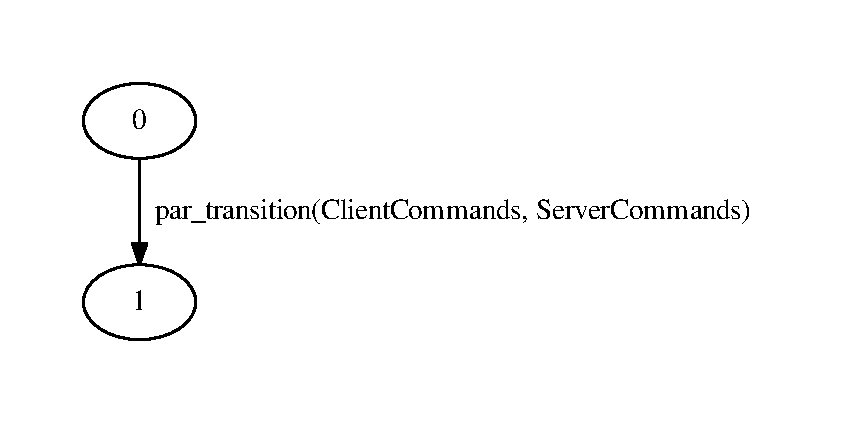
\includegraphics[width=0.4\textwidth]{chatsession_chatroom_dot.pdf}
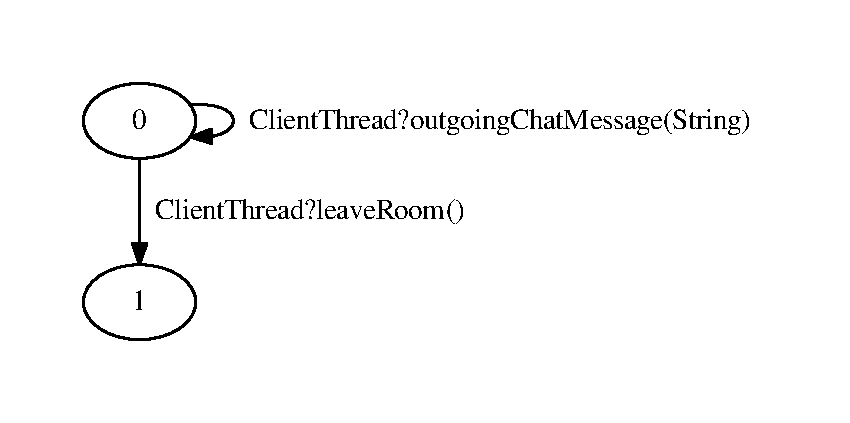
\includegraphics[width=0.4\textwidth]{chatsession_chatroom_dot_2.pdf} \\
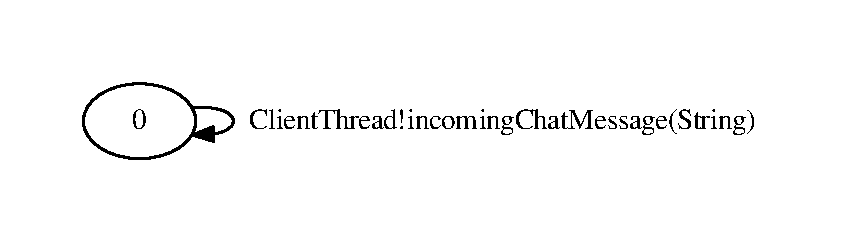
\includegraphics[width=0.4\textwidth]{chatsession_chatroom_dot_3.pdf}
\end{figure}

\subsection{ClientThread}
\begin{figure}[H]
\centering
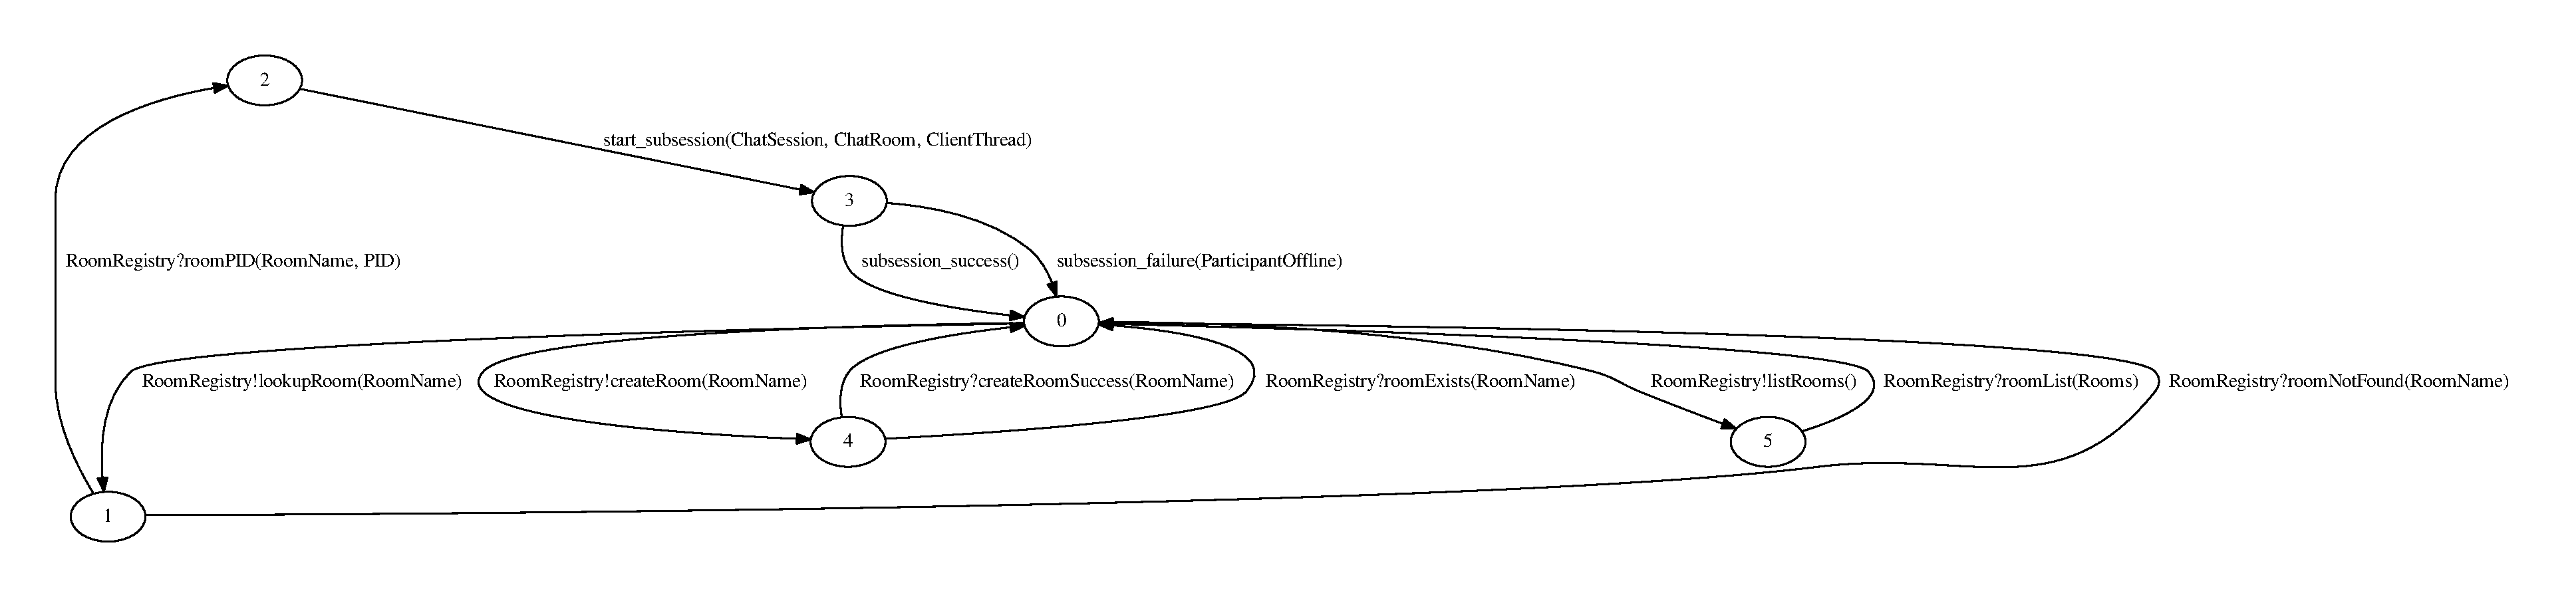
\includegraphics[width=\textwidth]{chatserver_clientthread_dot.pdf} \\
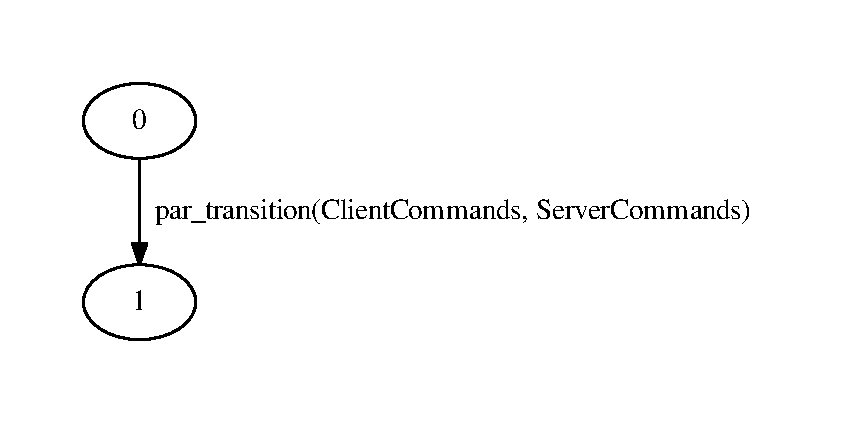
\includegraphics[width=0.4\textwidth]{chatsession_clientthread_dot.pdf}
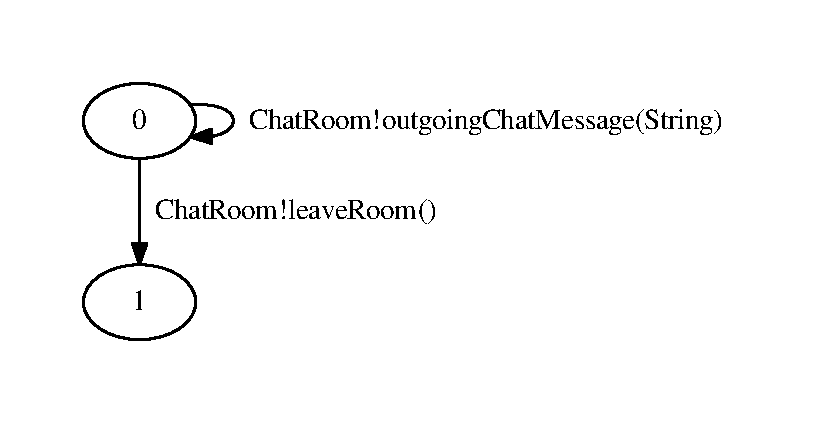
\includegraphics[width=0.4\textwidth]{chatsession_clientthread_dot_2.pdf} \\
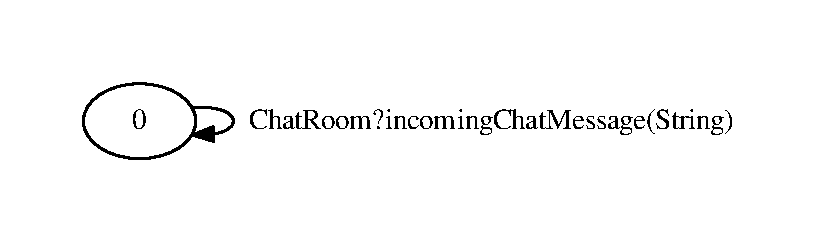
\includegraphics[width=0.4\textwidth]{chatsession_clientthread_dot_3.pdf}

\end{figure}

\subsection{RoomRegistry}
\begin{figure}[H]
\centering
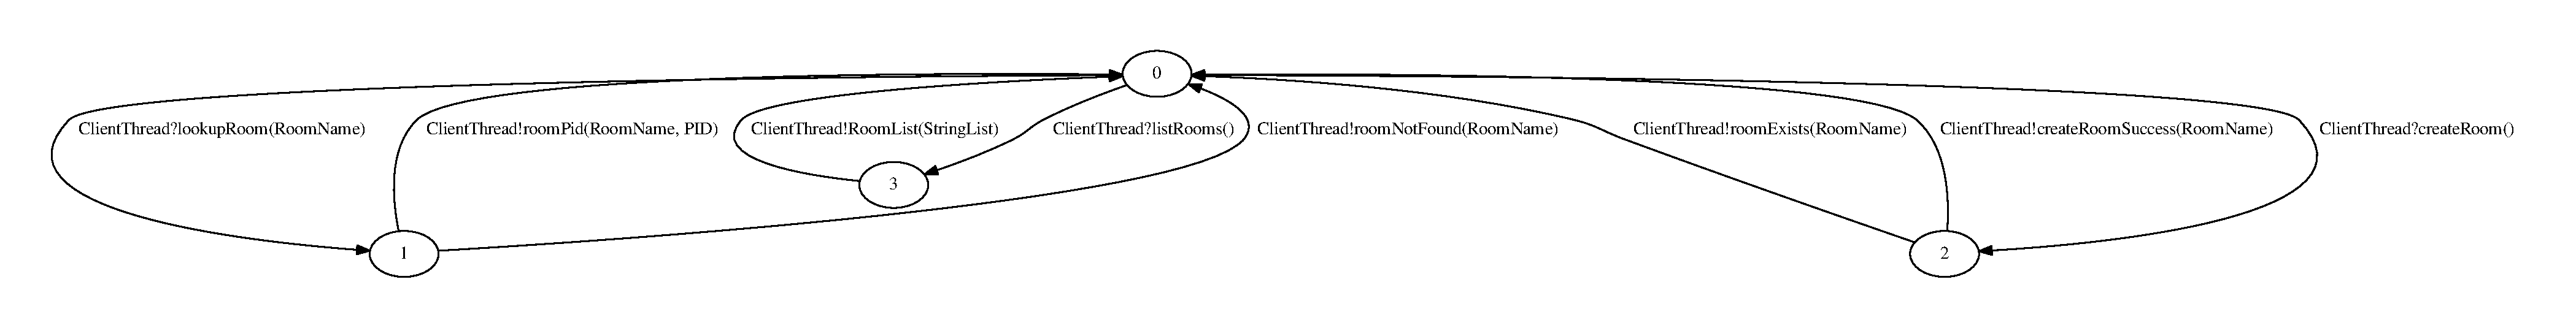
\includegraphics[width=\textwidth]{chatserver_roomregistry_dot.pdf}
\end{figure}

\section{Sequence Diagram}

\begin{figure}[H]
\centering
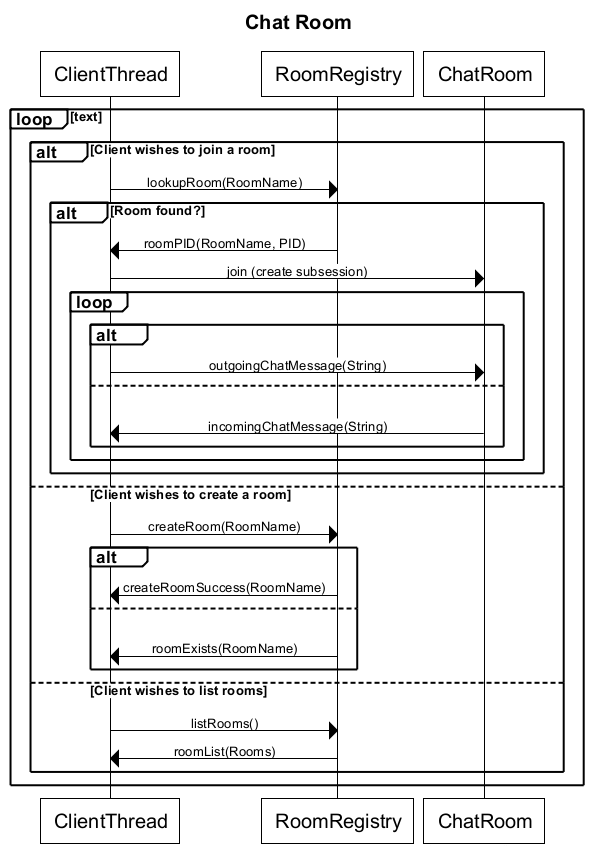
\includegraphics[width=0.8\textwidth]{Chat_Room.png}
\end{figure}

\bibliographystyle{plainnat}
\bibliography{simonfowler}
\end{document}